%% LyX 2.4.0~beta5 created this file.  For more info, see https://www.lyx.org/.
%% Do not edit unless you really know what you are doing.
\documentclass[french,english,footrule]{foils}
\usepackage[T1]{fontenc}
\usepackage[latin9]{inputenc}
\usepackage{geometry}
\geometry{verbose}
\setcounter{secnumdepth}{1}
\setcounter{tocdepth}{1}
\synctex=-1
\usepackage{xcolor}
\usepackage{babel}
\usepackage{fancybox}
\usepackage{calc}
\usepackage{url}
\usepackage{amsmath}
\usepackage{amsthm}
\usepackage{amssymb}
\usepackage{graphicx}
\usepackage[pdfusetitle,
 bookmarks=true,bookmarksnumbered=false,bookmarksopen=false,
 breaklinks=false,pdfborder={0 0 1},backref=false,colorlinks=false]
 {hyperref}

\makeatletter

%%%%%%%%%%%%%%%%%%%%%%%%%%%%%% LyX specific LaTeX commands.
\newcommand{\noun}[1]{\textsc{#1}}

%%%%%%%%%%%%%%%%%%%%%%%%%%%%%% Textclass specific LaTeX commands.
\newenvironment{lyxcode}
	{\par\begin{list}{}{
		\setlength{\rightmargin}{\leftmargin}
		\setlength{\listparindent}{0pt}% needed for AMS classes
		\raggedright
		\setlength{\itemsep}{0pt}
		\setlength{\parsep}{0pt}
		\normalfont\ttfamily}%
	 \item[]}
	{\end{list}}

%%%%%%%%%%%%%%%%%%%%%%%%%%%%%% User specified LaTeX commands.
\usepackage{graphicx,xcolor}
% darker colors for better slides...
\definecolor{green}{RGB}{0, 180, 0}
\definecolor{cyan}{RGB}{0, 180, 180}
\definecolor{yellow}{RGB}{211,211,0}

%\usepackage{xcolor}
\renewcommand{\labelitemi}{$\textcolor{blue}{\bullet}$}
\renewcommand{\labelitemii}{$\textcolor{teal}{\Rightarrow}$}
\renewcommand{\labelitemiii}{$\textcolor{red}{\rightarrow}$}
\renewcommand{\labelitemiv}{$\textcolor{brown}{\circ}$}

\newcommand{\T}{\mathrm{T}}  % transpose
\newcommand{\PP}{\mathrm{P}}  % probability
\newcommand{\dd}{\mathrm{d}} % integration dx
\newcommand{\ee}{\mathrm{e}} % exponential
\newcommand{\E}{\mathrm{E}} % expectation

\newcommand{\argmin}{\operatornamewithlimits{argmin}}

% bold vectors
\newcommand{\bu}{\mathbf{u}} 
\newcommand{\bU}{\mathbf{U}} 
\newcommand{\X}{\mathbf{X}}  
\newcommand{\x}{\mathbf{x}}  
\newcommand{\Ho}{\mathbf{H}}  
\newcommand{\bY}{\mathbf{Y}}  
\newcommand{\bP}{\mathbf{P}}  
\newcommand{\bA}{\mathbf{A}}  
\newcommand{\M}{\mathbf{M}}  
\newcommand{\B}{\mathbf{B}}  

% DA
\newcommand{\xf}{\mathbf{x}^{\mathrm{f}}}
\newcommand{\xa}{\mathbf{x}^{\mathrm{a}}}
\newcommand{\xb}{\mathbf{x}^{\mathrm{b}}}
\newcommand{\xt}{\mathbf{x}^{\mathrm{t}}}
\newcommand{\barx}{\overline{\mathbf{x}}}

%\newcommand{\x}{\mathbf{x}}
\newcommand{\y}{\mathbf{y}}
\newcommand{\yo}{\mathbf{y}^{\mathrm{o}}}
\newcommand{\bary}{\overline{\mathbf{y}}}

%\newcommand{\X}{\mathbf{X}}
\newcommand{\Xf}{\mathbf{X}_{\mathrm{f}}}
\newcommand{\Xa}{\mathbf{X}_{\mathrm{a}}}

%\newcommand{\bY}{\mathbf{Y}}
\newcommand{\Yf}{\mathbf{Y}_{\mathrm{f}}}

\newcommand{\w}{\mathbf{w}}
%\newcommand{\W}{\mathbf{W}}

\newcommand{\z}{\mathbf{z}}
\newcommand{\dv}{\mathbf{d}}

%\newcommand{\Pa}{\mathbf{P}^{\mathrm{a}}}
\newcommand{\Pf}{\mathbf{P}^{\mathrm{f}}}

%\newcommand{\K}{\mathbf{K}}
%\newcommand{\B}{\mathbf{B}}
\newcommand{\R}{\mathbf{R}}
\newcommand{\Q}{\mathbf{Q}}
%\newcommand{\Ho}{\mathbf{H}}
\newcommand{\Hc}{\mathcal{H}}

%\newcommand{\M}{\mathbf{M}}
\newcommand{\Mc}{\mathcal{M}}
\newcommand{\Mk}{\mathbf{M}_{k}}
\newcommand{\Mkk}{\mathbf{M}_{k+1}}

\newcommand{\Rn}{\mathbb{R}^{n}}
\newcommand{\Rp}{\mathbb{R}^{p}}
\newcommand{\Rm}{\mathbb{R}^{m}}
\newcommand{\Rnn}{\mathbb{R}^{n\times n}}
\newcommand{\Rpp}{\mathbb{R}^{p\times p}}
\newcommand{\Id}{\mathbf{I}}

\newcommand{\ea}{\boldsymbol{\epsilon}^{\mathrm{a}}}
\newcommand{\eb}{\boldsymbol{\epsilon}^{\mathrm{b}}}
\newcommand{\ef}{\boldsymbol{\epsilon}^{\mathrm{f}}}
\newcommand{\eo}{\boldsymbol{\epsilon}^{\mathrm{o}}}
\newcommand{\eq}{\boldsymbol{\epsilon}^{\mathrm{q}}}

\newcommand{\zero}{\mathbf{0}}
\newcommand{\one}{\mathbf{1}}
\newcommand{\onehalf}{\frac{1}{2}}


\newcommand{\nn}{\nonumber\\}
\newcommand{\tr}{\rm Tr}
\def\({\left(}
\def\){\right)}

%\newcommand{\bu}{\mathbf{u}}
\newcommand{\baru}{\overline{\mathbf{u}}}
\newcommand{\bh}{\mathbf{h}}
\newcommand{\bv}{\mathbf{v}}
\newcommand{\bz}{\mathbf{z}}

%\newcommand{\bP}{\mathbf{P}}
\newcommand{\bS}{\mathbf{S}}
%\newcommand{\bA}{\mathbf{A}}
\newcommand{\bV}{\mathbf{V}}
\newcommand{\bT}{\mathbf{T}}
%\newcommand{\bU}{\mathbf{U}}
\newcommand{\bE}{\mathbf{E}}
\newcommand{\bZ}{\mathbf{Z}}
\newcommand{\bC}{\mathbf{C}}
\newcommand{\bL}{\mathbf{L}}

\newcommand{\bOmega}{\mathbf{\Omega}}
\newcommand{\bLambda}{\mathbf{\Lambda}}
\newcommand{\bdelta}{\bm{\delta}}
\newcommand{\brho}{\boldsymbol{\rho}}
\newcommand{\beps}{\boldsymbol{\epsilon}}
\newcommand{\bSigma}{\mathbf{\Sigma}}
\newcommand{\balpha}{\boldsymbol{\alpha}}
%\newcommand{\bbeta}{\bm{\beta}}
%\newcommand{\btheta}{\bm{\theta}}
\newcommand{\ceta}{\boldsymbol{\eta}}

%%MB
\newcommand{\Hess}{\mathrm{H}}
\newcommand{\Tc}{\mathcal{T}}

%%MA
%\newcommand{\dd}{\mathrm{d}}
\newcommand{\Pb}{\mathbf{P}^{\mathrm{b}}}

\makeatother

\begin{document}
\title{Variational Data Assimilation\\
\rule[0.5ex]{1\columnwidth}{3pt}}
\author{Mark Asch - CSU/IMU/2023}
\date{\bigskip{}
\bigskip{}
\bigskip{}
\noun{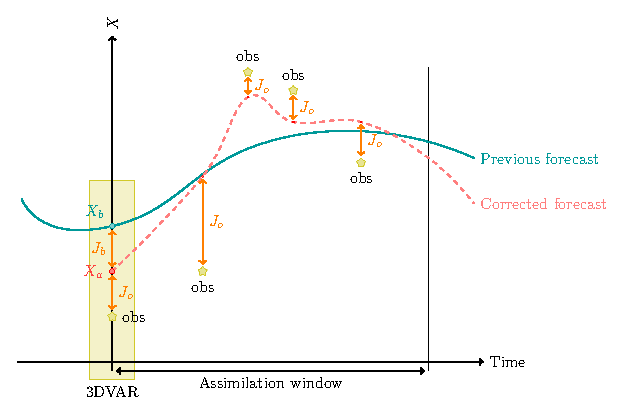
\includegraphics[scale=1.2]{graphics/3D4D-Var}}}
\maketitle

\MyLogo{Data Assim. 3-4D Var - M. Asch - Lecture 03}

\foilhead{Outline of the course (I)}

\textcolor{blue}{Adjoint methods and variational data assimilation
(4h)}
\begin{enumerate}
\item Introduction to data assimilation: setting, history, overview, definitions.
\item \textcolor{lightgray}{Adjoint method.}
\item \textcolor{red}{Variational data assimilation methods: }
\begin{enumerate}
\item \textcolor{red}{3D-Var, }
\item \textcolor{red}{4D-Var.}
\end{enumerate}
\end{enumerate}

\foilhead{Outline of the course (II)}

\textcolor{blue}{Statistical estimation, Kalman filters and sequential
data assimilation (4h)}
\begin{enumerate}
\item \textcolor{lightgray}{Introduction to statistical DA.
\item Statistical estimation.
\item The Kalman filter.
\item Nonlinear extensions and ensemble filters.}
\end{enumerate}

\foilhead{Reference Textbooks}
\begin{center}
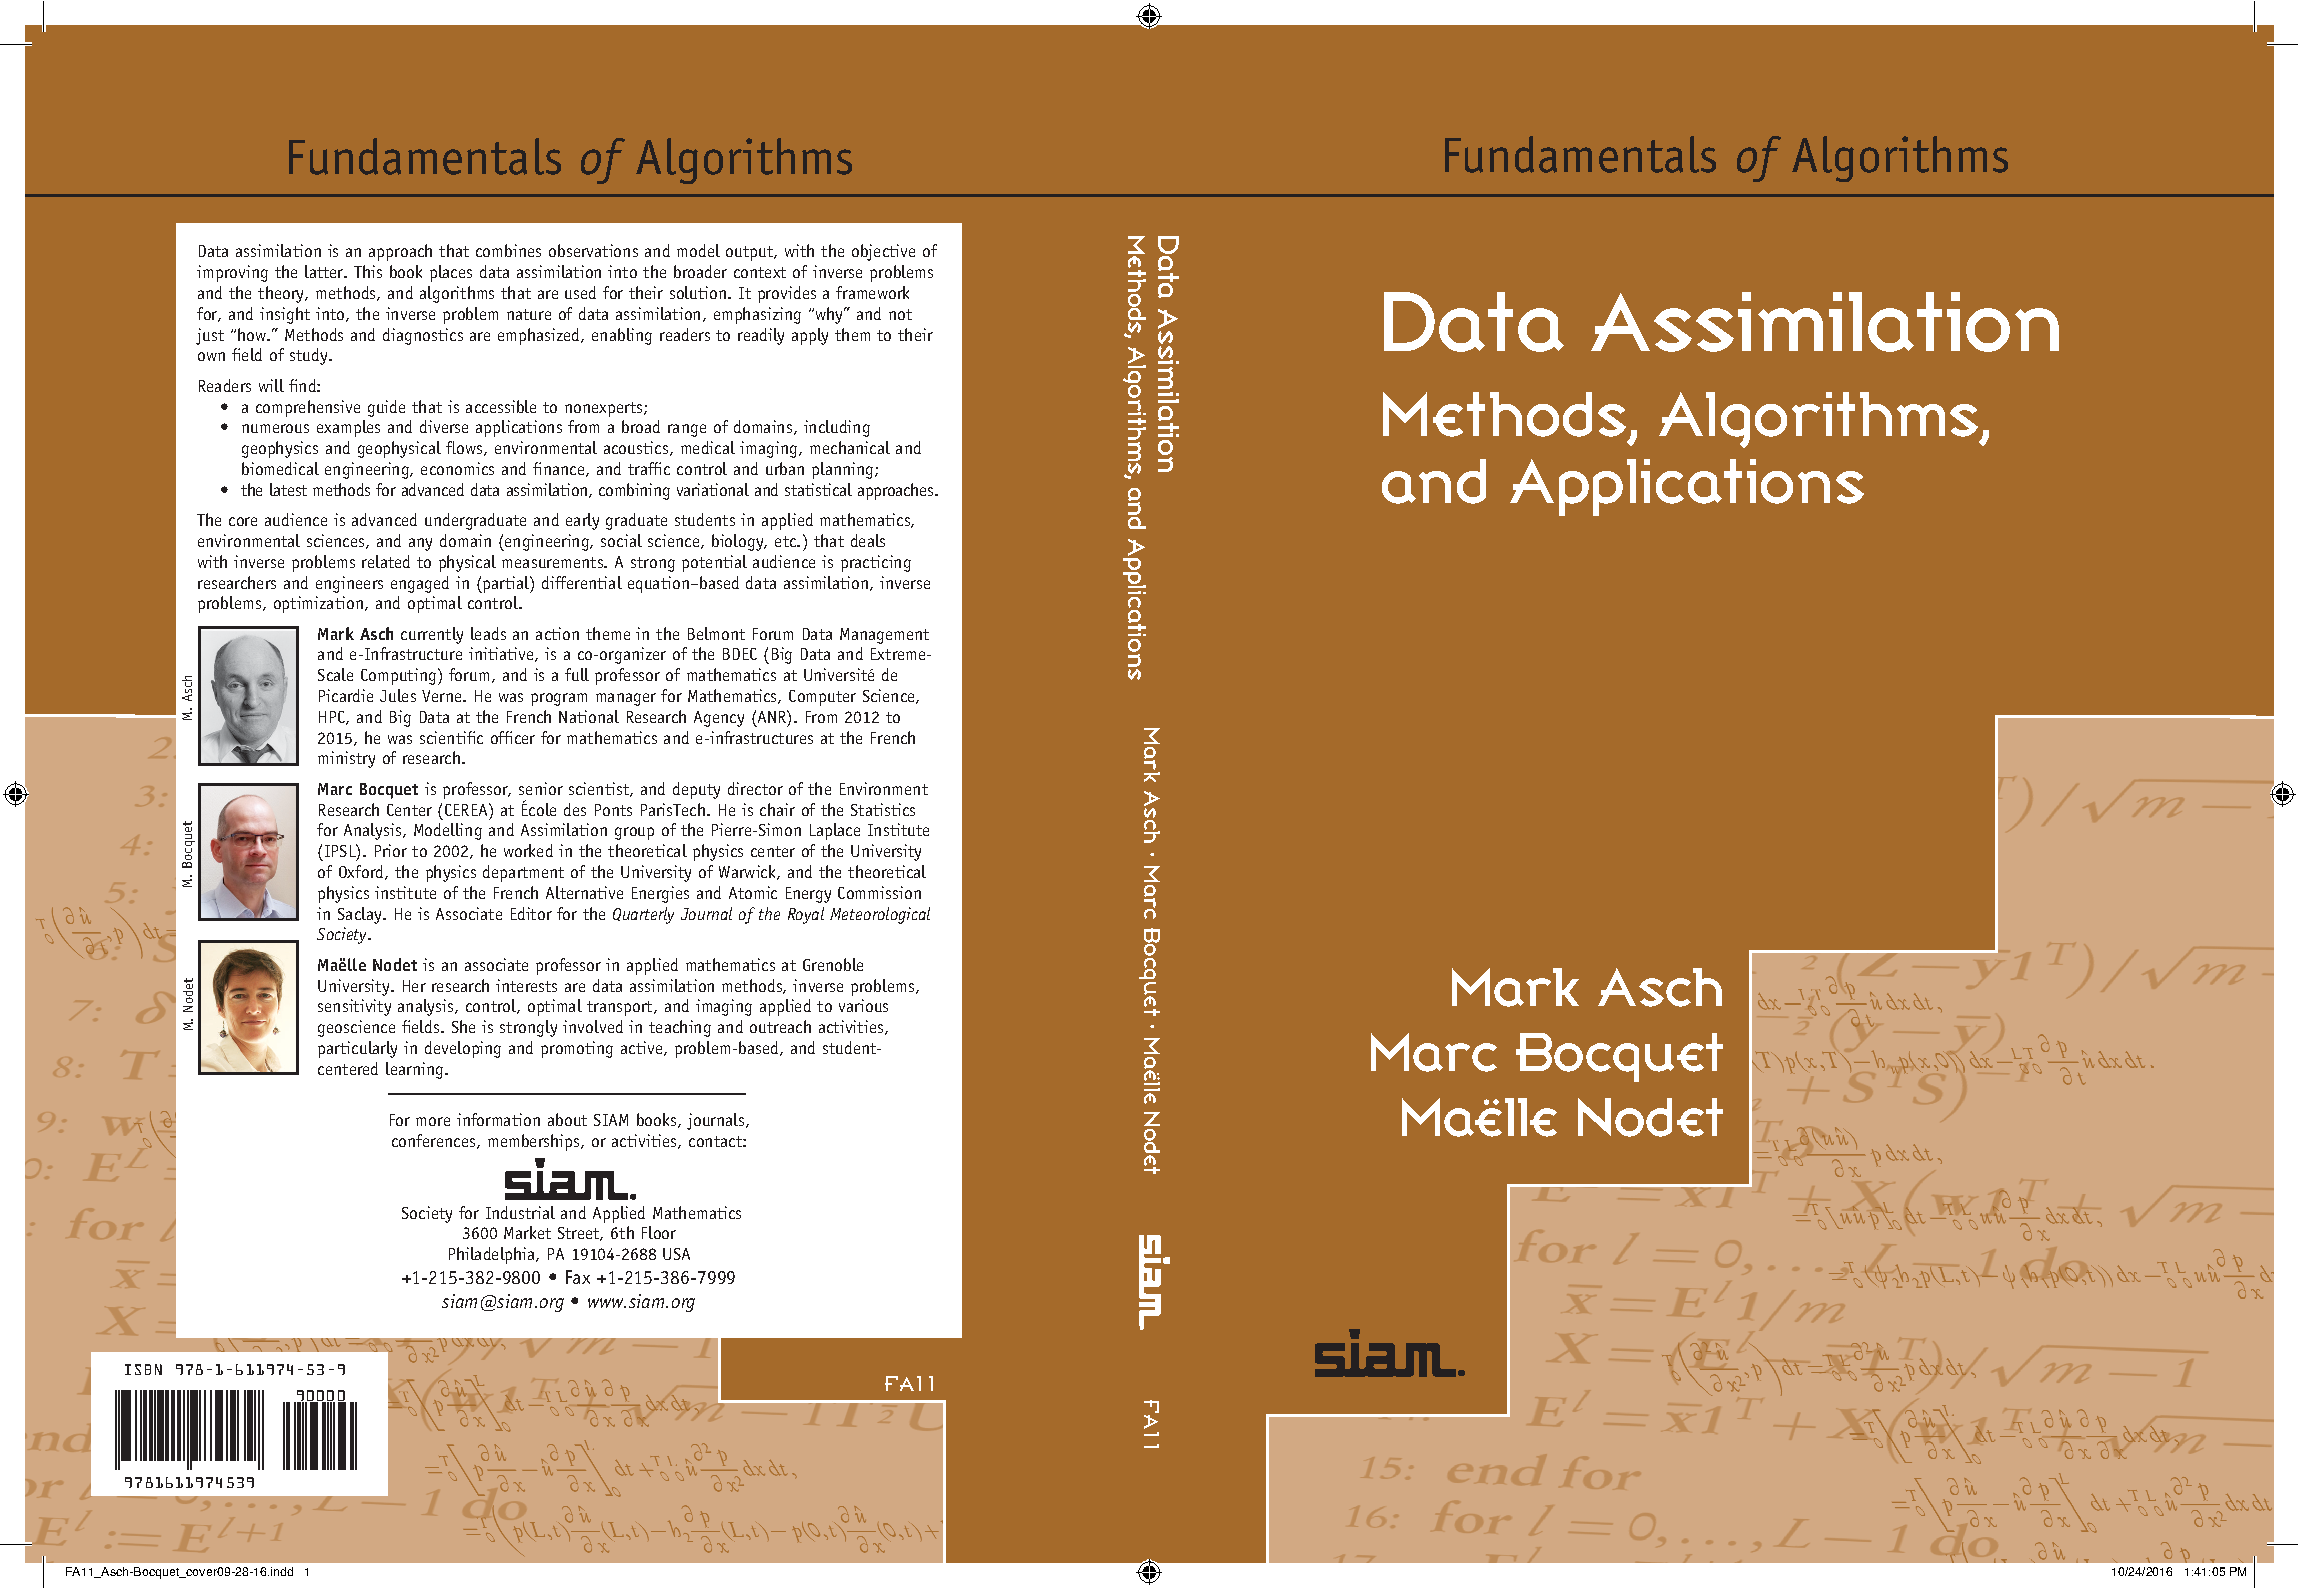
\includegraphics[width=0.8\textwidth]{graphics/FA11_Asch-Boucquet_cover10-24-16}
\par\end{center}

\begin{center}
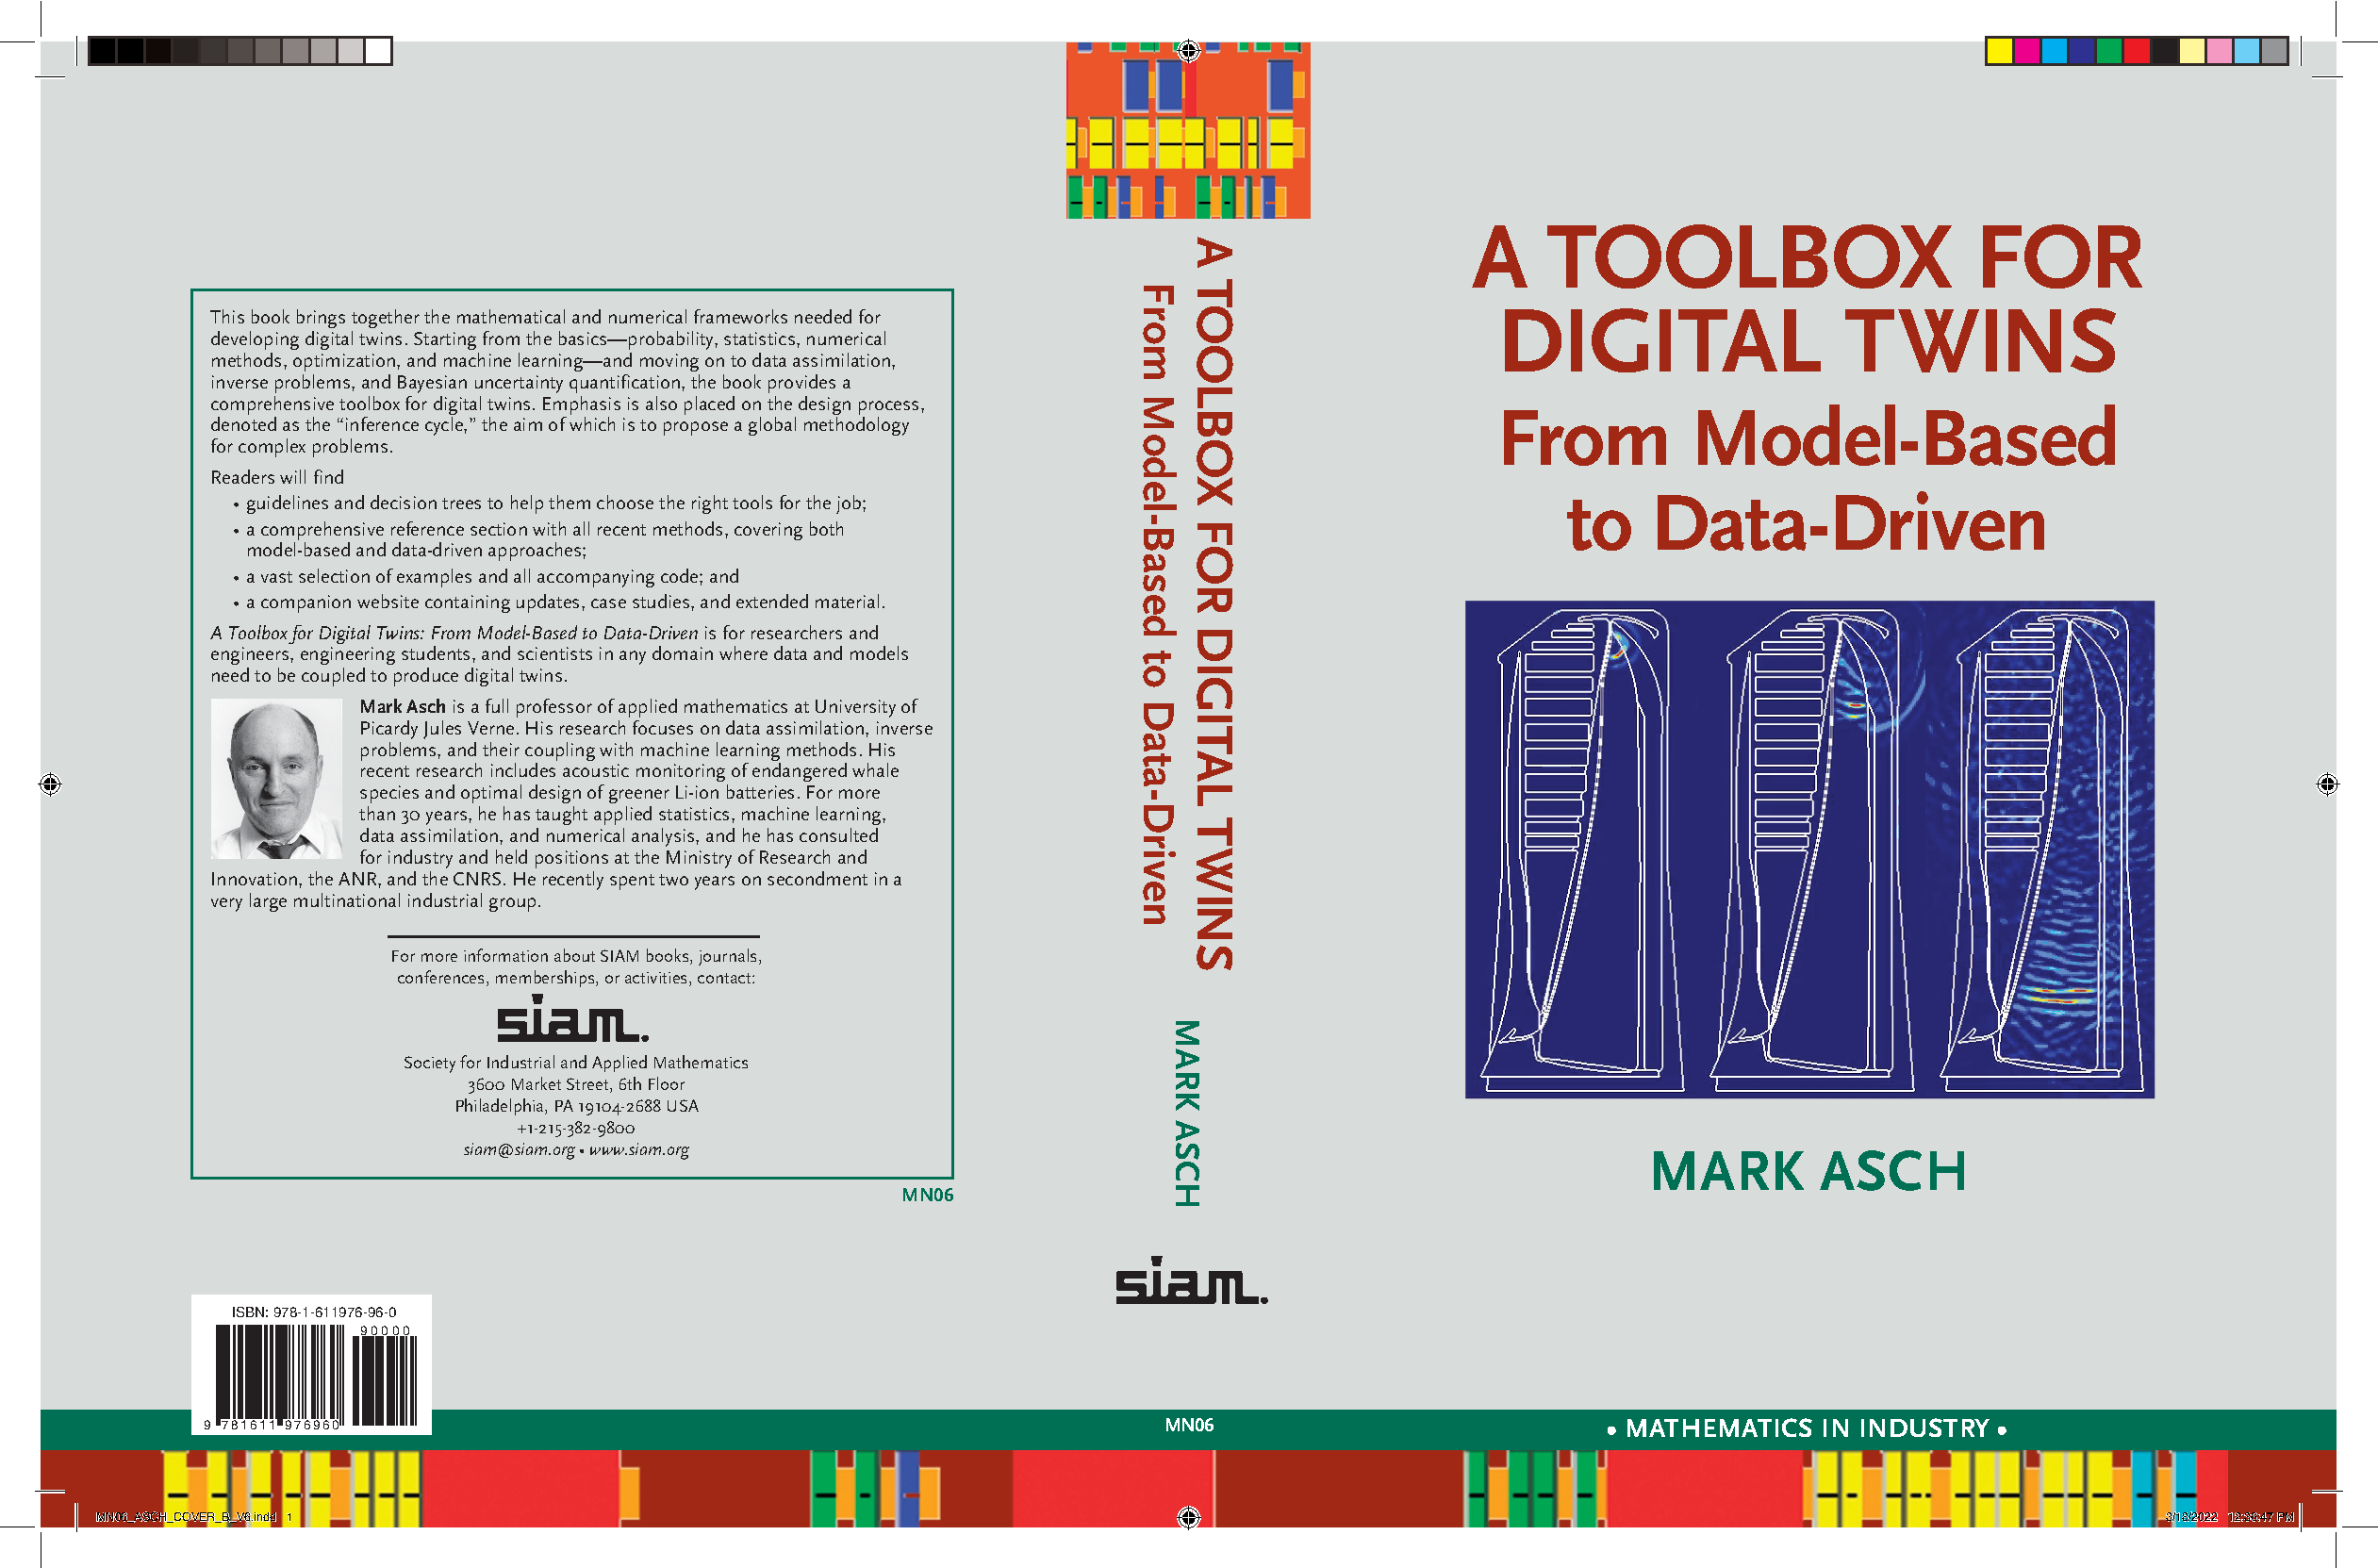
\includegraphics[width=0.8\textwidth]{graphics/MN06_ASCH_COVER_B_V6}
\par\end{center}

\foilhead{\textcolor{green}{Variational DA - formulation}}
\begin{itemize}
\item In variational data assimilation we describe the state of the system
by 
\begin{itemize}
\item a \textcolor{magenta}{state variable}, $\x(t)\in\mathcal{X},$ a function
of space and time that 
\item represents the physical variables of interest, such as current velocity
(in oceanography), temperature, sea-surface height, salinity, biological
species concentration, chemical concentration, etc. 
\end{itemize}
\item Evolution of the state is described by a system of (in general nonlinear)
\textcolor{magenta}{differential equations} in a region $\Omega,$
\begin{equation}
\left\{ \begin{aligned} & \frac{\mathrm{d}\x}{\mathrm{d}t}=\mathcal{M}(\x)\quad\mathrm{in}\;\Omega\times\left[0,T\right],\\
 & \x(t=0)=\x_{0},
\end{aligned}
\right.\label{eq:X-1}
\end{equation}
where the initial condition is unknown (or poorly known). 
\item Suppose that we are in possession of \textcolor{magenta}{observations}
$\mathbf{y}(t)\in\mathcal{O}$ and an observation \textcolor{magenta}{operator}
$\mathcal{H}$ that describes the available observations. 
\item Then, to characterize the difference between the observations and
the state, we define the \textcolor{magenta}{objective (or cost) function},
\begin{equation}
J(\x_{0})=\frac{1}{2}\int_{0}^{T}\left\Vert \mathbf{y}(t)-\mathcal{H}\left(\x(\x_{0},t)\right)\right\Vert _{\mathcal{O}}^{2}\mathrm{d}t+\frac{1}{2}\left\Vert \x_{0}-\x^{\mathrm{b}}\right\Vert _{\mathcal{X}}^{2},\label{eq:cf-1}
\end{equation}
where
\begin{itemize}
\item $\x^{\mathrm{b}}$ is the \textcolor{magenta}{background} (or first
guess) 
\item and the second term plays the role of a \textcolor{magenta}{regularization}
(in the sense of Tikhonov\textemdash see previous Lecture.\index{Tikhonov regularization (TR)!data assimilation} 
\item The two norms under the integral, in the finite-dimensional case,
will be represented by the \textcolor{magenta}{error covariance matrices}
$\mathbf{R}$ and $\mathbf{B}$ respectively, and will be described
below. 
\item Note that for mathematical rigor we have indicated, as subscripts,
the relevant functional spaces on which the norms are defined.
\end{itemize}
\item In the continuous context, the \textcolor{red}{data assimilation problem}
is formulated as follows: 
\end{itemize}
\selectlanguage{french}%
\noindent\shadowbox{\begin{minipage}[t]{1\columnwidth - 2\fboxsep - 2\fboxrule - \shadowsize}%
\selectlanguage{english}%
Find the analyzed state $\x_{0}^{\mathrm{a}}$ that minimizes $J$
and satisfies 
\[
\x_{0}^{\mathrm{a}}=\argmin J(\x_{0}).
\]
%
\end{minipage}}
\selectlanguage{english}%
\begin{itemize}
\item The \textcolor{magenta}{necessary condition} for the existence of
a (local) minimum is (as usual...)
\[
\nabla J(\x_{0}^{\mathrm{a}})=0.
\]
\end{itemize}

\foilhead{\textcolor{green}{Variational DA - adjoint method}}
\begin{itemize}
\item Variational DA is based on an\textcolor{magenta}{{} adjoint approach}
that is explained inthe previous Lecture. 
\item The particularity here is that the adjoint is used to solve an inverse
problem for the unknown \textcolor{magenta}{\emph{initial condition}}.
\end{itemize}

\foilhead{\textcolor{green}{Variational DA - 3D Var}}
\begin{itemize}
\item Usually, 3D-Var and 4D-Var are introduced in a finite dimensional
or discrete context\textemdash this approach will be used in this
section. 
\item For the infinite dimensional or continuous case, we must use the \textcolor{magenta}{calculus
of variations}\index{adjoint method!calculus of variations}\index{calculus of variations|see {adjoint method}}
and (partial) differential equations, as was done in the previous
Lectures.
\item We start out with the finite-dimensional version of the \textcolor{magenta}{cost
function} (\ref{eq:cf-1}), 
\begin{align}
J(\x) & =\frac{1}{2}\left(\x-\xb\right)^{\T}\B^{-1}\left(\x-\xb\right)\label{eq:cf_3dvar-1}\\
 & +\frac{1}{2}\left(\mathbf{Hx}-\mathbf{y}\right)^{\T}\R^{-1}\left(\mathbf{Hx}-\mathbf{y}\right),
\end{align}
where
\begin{itemize}
\item $\x,$ $\xb,$ and $\y$ are the \textcolor{magenta}{state}, the \textcolor{magenta}{background
state}, and the \textcolor{magenta}{measured state} respectively; 
\item $\Ho$ is the \textcolor{magenta}{observation matrix} (a linearization
of the observation operator $\mathcal{H}$ ); 
\item $\R$ and $\B$ are the observation and background \textcolor{magenta}{error
covariance matrices} respectively. 
\end{itemize}
\item This quadratic function attempts to strike a \textcolor{magenta}{balance}
between some \emph{a priori} knowledge about a \textcolor{magenta}{background}
(or historical) state and the actual measured, or \textcolor{magenta}{observed},
state. 
\item It also assumes that we know and that we can\textcolor{magenta}{{} invert
}the matrices $\mathbf{R}$ and $\mathbf{B}$. This, as we will be
pointed out below, is not always obvious. 
\item Furthermore, it represents the sum of the (weighted) background deviations
and the (weighted) observation deviations. The basic methodology is
presented in the Algorithm below, which is nothing more than a classical
\textcolor{magenta}{gradient descent} algorithm.
\end{itemize}

\foilhead{\textcolor{green}{Variational DA - 3D Var Algorithm}}
\begin{lyxcode}
$j=0$,~$x=x_{0}$

\textbf{while}~$\left\Vert \nabla J\right\Vert >\epsilon$~or~$j\le j_{\mathrm{max}}$

~~~~compute~$J$

~~~~compute~$\nabla J$

~~~~gradient~descent~and~update~of~$x_{j+1}$

~~~~$j=j+1$

\textbf{end}
\end{lyxcode}
\begin{center}
\noun{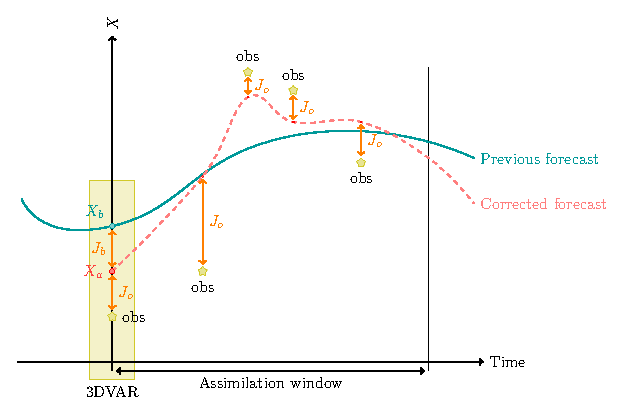
\includegraphics[scale=1.3]{graphics/3D4D-Var}}
\par\end{center}

\foilhead{\textcolor{green}{Variational DA - 3D Var (II)}}
\begin{itemize}
\item We note that when 
\begin{itemize}
\item the \textcolor{magenta}{background} $\x^{\mathrm{b}}=\x^{\mathrm{b}}+\epsilon^{\mathrm{b}}$
is available at some time $t_{k},$ together with 
\item \textcolor{magenta}{observations} of the form $\mathbf{y}=\mathbf{Hx}^{\mathrm{t}}+\epsilon^{\mathrm{o}}$
that have been acquired at the same time (or over a short enough interval
of time when the dynamics can be considered stationary), 
\item then the minimization of (\ref{eq:cf_3dvar-1}) will produce an \textcolor{magenta}{estimate
of the system state} at time $t_{k}.$ 
\end{itemize}
\item In this case, the analysis is called ``\textcolor{magenta}{three-dimensional
variational analysis}'' and is abbreviated by \textcolor{red}{\emph{3D-Var}}.
\item Borrowing from control theory\textemdash see {[}Asch2022{]}\textemdash the
\textcolor{magenta}{optimal gain}\index{3D-Var!optimal gain} can
be shown to take the form 
\[
\mathbf{K}=\B\Ho^{\T}(\Ho\B\Ho^{\T}+\R)^{-1},
\]
where $\B$ and $\R$ are the covariance matrices. 
\item We obtain the \textcolor{magenta}{analyzed state}, 
\[
\xa=\xb+\mathbf{K}(\y-\Ho(\xb)).
\]
\item This is the state that \textcolor{magenta}{minimizes} the \textcolor{magenta}{3D-Var
cost function}. 
\item We can verify this by taking the gradient, term by term, of the cost
function (\ref{eq:cf_3dvar-1}) and equating to zero, 
\begin{equation}
\nabla J(\xa)=\B^{-1}\left(\xa-\xb\right)-\Ho^{\T}\R^{-1}\left(\y-\Ho\xa\right)=0,\label{eq:gradJ3DVar}
\end{equation}
where 
\[
\xa=\argmin\,J(\x).
\]
\item Solving the equation, we find {\scriptsize
\begin{eqnarray}
\B^{-1}\left(\xa-\xb\right) & = & \Ho^{\T}\R^{-1}\left(\y-\Ho\xa\right)\nonumber \\
\left(\B^{-1}+\Ho^{\T}\R^{-1}\Ho\right)\xa & = & \Ho^{\T}\R^{-1}\y+\B^{-1}\xb\nonumber \\
\xa & = & \left(\B^{-1}+\Ho^{\T}\R^{-1}\Ho\right)^{-1}\left(\Ho^{\T}\R^{-1}\y+\B^{-1}\xb\right)\nonumber \\
 & = & \left(\B^{-1}+\Ho^{\T}\R^{-1}\Ho\right)^{-1}\left(\left(\B^{-1}+\Ho^{\T}\R^{-1}\Ho\right)\xb\right.\nonumber \\
 & ~ & \left.-\Ho^{\T}\R^{-1}\Ho\xb+\Ho^{\T}\R^{-1}\y\right)\nonumber \\
 & = & \xb+\left(\B^{-1}+\Ho^{\T}\R^{-1}\Ho\right)^{-1}\Ho^{\T}\R^{-1}\left(\y-\Ho\xb\right)\nonumber \\
 & = & \xb+\mathbf{K}\left(\y-\Ho\xb\right),\label{eq:lincontrol}
\end{eqnarray}
}where we have simply added and subtracted the term $\left(\Ho^{\T}\R^{-1}\Ho\right)\xb$
in the third-last line and in the last line we have brought out what
are known as the \textcolor{magenta}{\emph{innovation}}\index{innovation term}
term, 
\[
\dv=\y-\Ho\xb,
\]
and the \textcolor{magenta}{\emph{gain matrix}}, 
\[
\mathbf{K}=\left(\B^{-1}+\Ho^{\T}\R^{-1}\Ho\right)^{-1}\Ho^{\T}\R^{-1}.
\]
\item This matrix can be rewritten as 
\begin{equation}
\mathbf{K}=\B\Ho^{\T}\left(\R+\Ho\B\Ho^{\T}\right)^{-1}\label{eq:gain3DVAR}
\end{equation}
using a well-known Sherman-Morrison-Woodbury\index{Sherman-Morrison-Woodbury formula}
formula of linear algebra that completely avoids the direct computation
of the inverse of the matrix $\B.$ 
\item The linear combination in (\ref{eq:lincontrol}) of a background term
plus a multiple of the innovation is a classical result of\textcolor{magenta}{{}
linear-quadratic (LQ) control theory} and shows how nicely DA fits
in with and corresponds to (optimal) control theory
\item The form of the gain matrix (\ref{eq:gain3DVAR}) can be explained
quite simply.
\begin{itemize}
\item The term $\Ho\B\Ho^{\T}$ is the background covariance transformed
to the observation space. 
\item The ``denominator'' term $\R+\Ho\B\Ho^{\T}$ expresses the sum of
observation and background covariances. 
\item The ``numerator'' term $\B\Ho^{\T}$ takes the ratio of $\B$ and
$\R+\Ho\B\Ho^{\T}$ back to the model space. 
\end{itemize}
\item This recalls (and is completely analogous to) the variance ratio 
\[
\frac{\sigma_{\mathrm{b}}^{2}}{\sigma_{b}^{2}+\sigma_{\mathrm{o}}^{2}}
\]
that appears in the \textcolor{magenta}{optimal BLUE} (Best Linear
Unbiased Estimate)\index{best linear unbiased estimator (BLUE)!3D-Var}
that will be derived below in the \textcolor{magenta}{statistical
DA} Lecture. 
\item This corresponds to the case of a single observation $y^{\mathrm{o}}=x^{\mathrm{o}}$
of a quantity $x,$ 
\begin{eqnarray*}
x^{\mathrm{a}} & = & x^{\mathrm{b}}+\frac{\sigma_{\mathrm{b}}^{2}}{\sigma_{\mathrm{b}}^{2}+\sigma_{\mathrm{o}}^{2}}(x^{\mathrm{o}}-x^{\mathrm{b}})\\
 & = & x^{\mathrm{b}}+\frac{1}{1+\alpha}(x^{\mathrm{o}}-x^{\mathrm{b}}),
\end{eqnarray*}
where 
\[
\alpha=\frac{\sigma_{\mathrm{o}}^{2}}{\sigma_{\mathrm{b}}^{2}}.
\]
\item In other words, the best way to estimate the state is to take a \textcolor{magenta}{weighted
average} of the \textcolor{magenta}{background} (or prior) and the
\textcolor{magenta}{observations} of the state. And the best weight
is the ratio of the mean squared errors (\textcolor{magenta}{variances}). 
\item The statistical viewpoint is thus perfectly reproduced in the 3D-Var
framework.
\end{itemize}

\foilhead{\textcolor{green}{Variational DA - 4D Var}}
\begin{itemize}
\item \index{4D-Var|(} A more realistic, but complicated situation arises
when one wants to assimilate observations that are acquired over a
\textcolor{magenta}{time interval}, during which the system dynamics
(flow, for example) cannot be neglected. 
\item Suppose that the measurements are available at a succession of instants,
$t_{k},$ $k=0,1,\ldots,K$ and are of the form 
\begin{equation}
\y_{k}=\Ho_{k}\x_{k}+\eo_{k},\label{eq:4DvarObs}
\end{equation}
where 
\begin{itemize}
\item $\Ho_{k}$ is a linear \textcolor{magenta}{observation operator} and 
\item $\eo_{k}$ is the \textcolor{magenta}{observation error }with \textcolor{magenta}{covariance}
matrix $\R_{k},$ 
\item and suppose that these observation errors are \textcolor{magenta}{uncorrelated}
in time. 
\end{itemize}
\item Now we add the \textcolor{magenta}{dynamics} described by the\textcolor{magenta}{{}
state equation}, 
\begin{equation}
\x_{k+1}=\M_{k+1}\x_{k},\label{eq:4DvarState}
\end{equation}
where we have neglected any model error.\footnote{This will be taken into account below.} 
\item We suppose also that at time index $k=0$ we know 
\begin{itemize}
\item the \textcolor{magenta}{background} state $\xb_{0}$ and 
\item its error\textcolor{magenta}{{} covariance} matrix $\Pb_{0}$ 
\item and we suppose that the errors are uncorrelated with the observations
in (\ref{eq:4DvarObs}). 
\end{itemize}
\item Then a given initial condition, $\x_{0},$ defines a unique model
solution $\x_{k+1}$ according to (\ref{eq:4DvarState}). 
\item We can now generalize the\textcolor{magenta}{{} objective function}
(\ref{eq:cf_3dvar-1}), which becomes 
\begin{align}
J(\x_{0}) & =\frac{1}{2}\left(\x_{0}-\xb_{0}\right)^{\T}\left(\Pb_{0}\right)^{-1}\left(\x_{0}-\xb_{0}\right)\label{eq:4DvarObjStrong}\\
 & +\frac{1}{2}\sum_{k=0}^{K}\left(\Ho_{k}\x_{k}-\y_{k}\right)^{\T}\R_{k}^{-1}\left(\Ho_{k}\x_{k}-\y_{k}\right).
\end{align}
\item The \textcolor{magenta}{minimization} of $J(\x_{0})$ will provide
the \textcolor{magenta}{initial condition} of the model that fits
the data most closely. 
\item This analysis is called ``\textcolor{magenta}{strong constraint four-dimensional
variational assimilation},'' abbreviated as \textcolor{magenta}{\emph{strong
constraint 4D-Var}}\index{4D-Var!strong constraint}. The term ``strong
constraint'' implies that the model found by the state equation (\ref{eq:4DvarState})
must be exactly satisfied by the sequence of estimated state vectors.
\item In the presence of \textcolor{magenta}{model uncertainty}, the state
equation becomes 
\begin{equation}
\x_{k+1}^{\mathrm{t}}=\M_{k+1}\x_{k}^{\mathrm{t}}+\boldsymbol{\eta}_{k+1},\label{eq:mod_uncert}
\end{equation}
where 
\begin{itemize}
\item the model noise $\boldsymbol{\eta}_{k}$ has covariance matrix $\mathbf{Q}_{k},$ 
\item which we suppose to be uncorrelated in time and uncorrelated with
the background and observation errors. 
\end{itemize}
\item The \textcolor{magenta}{objective function} for the best, linear unbiased
estimator (\textcolor{magenta}{BLUE})\index{best linear unbiased estimator (BLUE)!4D-Var}
for the sequence of states 
\[
\left\{ \x_{k},\,k=0,1,\ldots,K\right\} 
\]
is of the form {\small
\begin{eqnarray}
J(\x_{0},\x_{1},\cdots,\x_{K})=\frac{1}{2}\left(\x_{0}-\x_{0}^{\mathrm{b}}\right)^{\T}\left(\mathbf{P}_{0}^{\mathrm{b}}\right)^{-1}\left(\x_{0}-\x_{0}^{\mathrm{b}}\right)\nonumber \\
+\frac{1}{2}\sum_{k=0}^{K}\left(\mathbf{H}_{k}\x_{k}-\mathbf{y}_{k}\right)^{\T}\mathbf{R}_{k}^{-1}\left(\mathbf{H}_{k}\x_{k}-\mathbf{y}_{k}\right)\nonumber \\
+\frac{1}{2}\sum_{k=0}^{K-1}\left(\x_{k+1}-\mathbf{M}_{\mathit{k}+1}\x_{k}\right)^{\T}\mathbf{Q}_{k+1}^{-1}\left(\x_{k+1}-\mathbf{M}_{\mathit{k}+1}\x_{k}\right).\label{eq:4DvarObj}
\end{eqnarray}
}{\small\par}
\item This objective function has become a function of the complete sequence
of states 
\[
\left\{ \x_{k},\,k=0,1,\ldots,K\right\} ,
\]
and its minimization is known as ``\textcolor{magenta}{weak constraint
four-dimensional variational assimilation},'' abbreviated as \emph{weak
constraint 4D-Var}\index{4D-Var!weak constraint}. 
\item Equations (\ref{eq:4DvarObjStrong}) and (\ref{eq:4DvarObj}), with
an appropriate reformulation of the state and observation spaces,
are special cases of the \textcolor{magenta}{BLUE} objective function.
\end{itemize}

\foilhead{\textcolor{green}{Variational DA - 4D Var Applications}}
\begin{itemize}
\item All the above forms of variational assimilation, as defined by (\ref{eq:cf_3dvar-1}),
(\ref{eq:4DvarObjStrong}) and (\ref{eq:4DvarObj}), have been used
for real-world data assimilation, in particular in meteorology and
oceanography. 
\item However, these methods are directly applicable to a \textcolor{magenta}{vast
array of other domains}, among which we can cite 
\begin{itemize}
\item geophysics and environmental sciences, 
\item seismology, 
\item atmospheric chemistry, and terrestrial magnetism.
\item Many other examples exist.
\end{itemize}
\item We remark that in real-world practice, variational assimilation is
performed on \textcolor{magenta}{nonlinear} models. If the extent
of the nonlinearity is sufficiently small (in some sense), then variational
assimilation, even if it does not solve the correct estimation problem,
will still produce useful results.
\end{itemize}

\foilhead{\textcolor{green}{Variational DA - 4D Var Implementation}}
\begin{itemize}
\item Now, our problem reduces to 
\begin{itemize}
\item quantifying the \textcolor{magenta}{covariance} matrices and then,
of course, 
\item computing the \textcolor{magenta}{analyzed} state. 
\end{itemize}
\item The quantification of the covariance matrices must result from extensive
data studies, or the use of a Kalman filter approach\textemdash see
below. 
\item The computation of the analyzed state will be described next\textemdash this
will not be done directly, but rather by an \textcolor{magenta}{adjoint
approach} for minimizing the cost functions. 
\item There is of course the inverse of $\B$ or $\mathbf{P}^{\mathrm{b}}$
to compute, but we remark that there appear only\textcolor{magenta}{{}
matrix-vector products} of $\B^{-1}$ and $\left(\mathbf{P}^{\mathrm{b}}\right)^{-1}$
and we can thus define operators (or routines) that compute these
efficiently without the need for large storage capacities.
\end{itemize}

\foilhead{\textcolor{green}{Variational DA - 4D Var Adjoint}}
\begin{itemize}
\item We explain the adjoint approach in the case of \textcolor{magenta}{strong
constraint 4D-Var,} taking into account a completely general nonlinear
setting for the model and for the observation operators. 
\item Let $\M_{k}$ and $\Ho_{k}$ be the nonlinear model and observation
operators respectively. 
\item We reformulate (\ref{eq:4DvarState}) and (\ref{eq:4DvarObjStrong})
in terms of the nonlinear operators as {\small
\begin{eqnarray}
J(\x_{0}) & = & \frac{1}{2}\left(\x_{0}-\xb_{0}\right)^{\T}\left(\bP_{0}^{\mathrm{b}}\right)^{-1}\left(\x_{0}-\xb_{0}\right)\nonumber \\
 &  & +\frac{1}{2}\sum_{k=0}^{K}\left(\Ho_{k}(\x_{k})-\y_{k}\right)^{\T}\R_{k}^{-1}\left(\Ho_{k}(\x_{k})-\y_{k}\right),\label{eq:4Dvar ObjNL}
\end{eqnarray}
}with the dynamics 
\begin{equation}
\x_{k+1}=\Mkk\left(\x_{k}\right),\quad k=0,1,\ldots,K-1.\label{eq:4DvarStateNL}
\end{equation}
\item The minimization problem requires that we now compute the gradient
of $J$ with respect to $\x_{0}.$ 
\item The gradient is determined from the property that, for a given perturbation
$\delta\x_{0}$ of $\x_{0},$ the corresponding first-order variation
of $J$ is 
\begin{equation}
\delta J=\left(\nabla_{\x_{0}}J\right)^{\T}\delta\x_{0}.\label{eq:4DvarVar}
\end{equation}
\item The perturbation is propagated by the tangent linear equation, 
\begin{equation}
\delta\x_{k+1}=\M_{k+1}\delta\x_{k},\quad k=0,1,\ldots,K-1,\label{eq:4DvarTLM}
\end{equation}
obtained by differentiation of the state equation (\ref{eq:4DvarStateNL}),
where $\M_{k+1}$ is the Jacobian matrix (of first-order partial derivatives)
of $\x_{k+1}$ with respect to $\x_{k}.$ 
\item The first-order variation of the cost function is obtained similarly
by differentiation of (\ref{eq:4Dvar ObjNL}), 
\begin{align}
\delta J & =\left(\x_{0}-\xb_{0}\right)^{\T}\left(\Pb_{0}\right)^{-1}\delta\x_{0}\label{eq:4DvarVarObj}\\
 & +\sum_{k=0}^{K}\left(\Ho_{k}(\x_{k})-\y_{k}\right)^{\T}\R_{k}^{-1}\Hess_{k}\delta\x_{k},
\end{align}
where $\Hess_{k}$ is the Jacobian of $\Ho_{k}$ and $\delta\x_{k}$
is defined by (\ref{eq:4DvarTLM}). 
\begin{itemize}
\item This variation is a compound function of $\delta\x_{0}$ that depends
on all the $\delta\x_{k}$'s. 
\item But if we can obtain a direct dependence on $\delta\x_{0}$ in the
form of (\ref{eq:4DvarVar}), eliminating the explicit dependence
on $\delta\x_{k},$ then we will (as in the previously seen examples)
arrive at an explicit expression for the gradient $\nabla_{\x_{0}}J$
of our cost function $J.$ 
\item This will be done, as we have done before, by introducing an adjoint
state and requiring that it satisfy certain conditions\textemdash namely,
the adjoint equation. Let us now proceed with this program.
\end{itemize}
\item We begin by defining, for $k=0,1,\ldots,K,$ the adjoint state vectors
$\mathbf{p}_{k}$ that belong to the dual of the state space. 
\item Now we take the null products (according to the tangent state equation
(\ref{eq:4DvarTLM})), 
\[
\mathbf{p}_{k}^{\T}\left(\delta\ \mathbf{x}_{k}-\M_{k}\delta\x_{k-1}\right),
\]
and subtract them from the right-hand side of the cost function variation
(\ref{eq:4DvarVarObj}), 
\begin{align*}
\delta J & =\left(\x_{0}-\xb_{0}\right)^{\T}\left(\Pb_{0}\right)^{-1}\delta\\
 & \x_{0}+\sum_{k=0}^{K}\left(\Ho_{k}(\x_{k})-\mathbf{y}_{k}\right)^{\T}\mathbf{R}_{k}^{-1}\Hess_{k}\delta\x_{k}\\
 & -\sum_{k=0}^{K}\mathbf{p}_{k}^{\T}\left(\delta\x_{k}-\mathbf{M}_{k}\delta\x_{k-1}\right).
\end{align*}
\item Rearranging the matrix products, using the symmetry of $\mathbf{R}_{k}$
and regrouping terms in $\delta\x_{\cdot},$ we obtain, {\footnotesize
\begin{eqnarray*}
\delta J & = & \left[\left(\mathbf{P}_{0}^{\mathrm{b}}\right)^{-1}\left(\x_{0}-\xb_{0}\right)+\Hess_{0}^{\T}\mathbf{R}_{0}^{-1}\left(\Ho_{0}(\x_{0})-\mathbf{y}_{0}\right)+\mathbf{M}_{0}^{\T}\mathbf{p}_{1}\right]\delta\x_{0}\\
 &  & +\left[\sum_{k=1}^{K-1}\Hess_{k}^{\T}\mathbf{R}_{k}^{-1}\left(\Ho_{k}(\x_{k})-\mathbf{y}_{k}\right)-\mathbf{p}_{k}+\mathbf{M}_{k}^{\T}\mathbf{p}_{k+1}\right]\delta\x_{k}\\
 &  & +\left[\Hess_{K}^{\T}\mathbf{R}_{K}^{-1}\left(\Ho_{K}(\x_{K})-\mathbf{y}_{K}\right)-\mathbf{p}_{K}\right]\delta\x_{k}.
\end{eqnarray*}
}{\footnotesize\par}
\item Notice that this expression is valid for any choice of the adjoint
states $\mathbf{p}_{k}$ and, in order to ``kill'' all $\delta\x_{k}$
terms, except $\delta\x_{0},$ we must simply impose that, {\footnotesize
\begin{eqnarray}
\mathbf{p}_{K} & = & \Hess_{K}^{\T}\mathbf{R}_{K}^{-1}\left(\Ho_{K}(\x_{K})-\mathbf{y}_{K}\right),\label{eq:4DvarAdj1}\\
\mathbf{p}_{k} & = & \Hess_{k}^{\T}\mathbf{R}_{k}^{-1}\left(\Ho_{k}(\x_{k})-\mathbf{y}_{k}\right)+\mathbf{M}_{k}^{\T}\mathbf{p}_{k+1},\quad k=K-1,\ldots,1,\label{eq:4DvarAdj2}\\
\mathbf{p}_{0} & = & \left(\mathbf{P}_{0}^{\mathrm{b}}\right)^{-1}\left(\x_{0}-\x_{0}^{\mathrm{b}}\right)+\Hess_{0}^{\T}\mathbf{R}_{0}^{-1}\left(\Ho_{0}(\x_{0})-\mathbf{y}_{0}\right)+\mathbf{M}_{0}^{\T}\mathbf{p}_{1}.\label{eq:4DvarAdj3}
\end{eqnarray}
}{\footnotesize\par}
\item We recognize the backward, adjoint equation for $\mathbf{p}_{k}$
and the only term remaining in the variation of $J$ is then 
\[
\delta J=\mathbf{p}_{0}^{\T}\delta\x_{0},
\]
so that $\mathbf{p}_{0}$ is the sought for gradient, $\nabla_{\x_{0}}J$,
of the objective function with respect to the initial condition $\x_{0}$
according to (\ref{eq:4DvarVar}). 
\item The system of equations (\ref{eq:4DvarAdj1})-(\ref{eq:4DvarAdj3})
is the adjoint of the tangent linear equation (\ref{eq:4DvarTLM}).
\item The term \emph{adjoint} here corresponds to the transposes of the
matrices $\Hess_{k}^{\T}$ and $\mathbf{M}_{k}^{\T}$ that, as we
have seen before, are the finite-dimensional analogues of an adjoint
operator. 
\end{itemize}

\foilhead{\textcolor{green}{Variational DA - 4D Var Algorithm}}
\begin{itemize}
\item We can now propose the ``usual'' algorithm for solving the optimization
problem by the adjoint approach:
\end{itemize}
\begin{enumerate}
\item For a given initial condition $\x_{0},$ integrate forwards the (nonlinear)
state equation (\ref{eq:4DvarStateNL}) and store the solutions $\x_{k}$
(or use some sort of checkpointing). 
\item From the final condition, (\ref{eq:4DvarAdj1}), integrate backwards
in time the adjoint equations (\ref{eq:4DvarAdj2}). 
\item Compute directly the required gradient (\ref{eq:4DvarAdj3}). 
\item Use this gradient in an iterative optimization algorithm to find a
(local) minimum. 
\end{enumerate}
\begin{itemize}
\item The above description for the solution of the 4D-Var data assimilation
problem clearly covers the case of 3D-Var,\index{adjoint method!3D-Var}
where we seek to minimize (\ref{eq:cf_3dvar-1}). In this case, we
only need the transpose Jacobian $\Hess^{\T}$ of the observation
operator. \index{4D-Var|)}
\end{itemize}

\foilhead{\textcolor{green}{Variational DA - roles of $\R$ and $\B$}}
\begin{itemize}
\item The \textcolor{magenta}{relative magnitudes} of the \textcolor{magenta}{errors}
due to measurement and background provide us with important information
as to how much ``weight'' to give to the different information sources
when solving the assimilation problem. 
\item For example, if background errors are larger than observation errors,
then the analyzed state, solution to the DA problem, should be closer
to the observations than to the background and vice-versa.
\item The \textcolor{magenta}{background error} covariance matrix, $\B,$
plays an important role in DA. This is illustrated in the following
examples.
\end{itemize}

\foilhead{$\;$}

\vfill{}

\begin{center}
{\Large\textbf{\textcolor{blue}{3D- and 4D-VAR EXAMPLES}}}{\Large\par}
\par\end{center}

\vfill{}


\foilhead{\textcolor{blue}{3D-VAR - effect of a single observation}}
\begin{itemize}
\item Suppose that we have a \textcolor{magenta}{single observation}, at
a point corresponding to the $j$-th element of the state vector. 
\item The \textcolor{magenta}{observation operator} is then 
\[
\Ho=(\begin{array}{ccccccc}
0 & \cdots & 0 & 1 & 0 & \cdots & 0\end{array})^{\T}.
\]
\item The \textcolor{magenta}{gradient} of $J$ is 
\[
\nabla J=\B^{-1}\left(\x-\xb\right)+\Ho^{\T}\R^{-1}\left(\Ho\x-\yo\right).
\]
\item Since it must be equal to zero at the minimum $\xa,$ we must have
\[
\left(\xa-\xb\right)=\B\Ho^{\T}\R^{-1}\left(\yo-\Ho\xa\right).
\]
\item But $\R\doteq\sigma^{2},$ $\Ho\xa=x_{j}^{\mathrm{a}}$ and $\B\Ho^{\T}$
is the $j$-th column of $\B$ whose elements are denoted by $B_{i,j}$
with $i=1,\ldots,n.$ 
\item So we see that 
\[
\xa-\xb=\frac{y^{\mathrm{o}}-x_{k}^{\mathrm{a}}}{\sigma^{2}}\left(\begin{array}{c}
B_{1,j}\\
B_{2,j}\\
\vdots\\
B_{n,j}
\end{array}\right).
\]
\item The increment is proportional to a column of $\B.$ 
\item The choice of $\B$ is thus crucial and will determine how this observation
provides information about what happens around the $j$-th variable.
\item In the \textcolor{magenta}{4D-Var case}, the increment at time $t$
will be proportional to a single column of $\M\B\M^{\T}$ which describes
the error covariances of the background at the time of the observation
$t.$
\end{itemize}

\foilhead{\textcolor{blue}{4D-VAR - for a single observation}}
\begin{itemize}
\item We consider an example with 
\begin{itemize}
\item a \textcolor{magenta}{single observation} at time step $3$ 
\item and a\textcolor{magenta}{{} known background }at time step $0.$ 
\end{itemize}
\item In this case, the\textcolor{magenta}{{} 4D-Var cost function} (\ref{eq:4DvarObjStrong})
for determining the initial state becomes scalar, 
\[
J(x_{0})=\frac{1}{2}\frac{\left(x_{0}-x_{0}^{\mathrm{b}}\right)^{2}}{\sigma_{B}^{2}}+\frac{1}{2}\sum_{k=1}^{K}\frac{\left(x_{k}-x_{k}^{\mathrm{o}}\right)^{2}}{\sigma_{R}^{2}},
\]
where $\sigma_{B}^{2}$ and $\sigma_{R}^{2}$ are the (known) \textcolor{magenta}{background}
and \textcolor{magenta}{observation error variances} respectively. 
\item With a single observation, say at time step $3$, the \textcolor{magenta}{cost
function} is 
\[
J(x_{0})=\frac{1}{2}\frac{\left(x_{0}-x_{0}^{\mathrm{b}}\right)^{2}}{\sigma_{B}^{2}}+\frac{1}{2}\frac{\left(x_{3}-x_{3}^{\mathrm{o}}\right)^{2}}{\sigma_{R}^{2}}.
\]
\item The \textcolor{magenta}{minimum} is reached when the gradient of $J$
disappears, 
\[
J'(x_{0})=0,
\]
which can be computed as 
\begin{equation}
\frac{\left(x_{0}-x_{0}^{\mathrm{b}}\right)}{\sigma_{B}^{2}}+\frac{\left(x_{3}-x_{3}^{\mathrm{o}}\right)}{\sigma_{R}^{2}}\frac{\dd x_{3}}{\dd x_{2}}\frac{\dd x_{2}}{\dd x_{1}}\frac{\dd x_{1}}{\dd x_{0}}=0.\label{eq:nec_scalar}
\end{equation}
\item We now require a \textcolor{magenta}{dynamic relation} between the
$x_{k}$'s in order to compute the derivatives. 
\item To this end, let us take the most simple\textcolor{magenta}{{} linear
forecast model}, 
\[
\frac{\dd x}{\dd t}=-\alpha x,
\]
with $\alpha$ a known positive constant. 
\item This is a typical model for describing decay, for example of a chemical
compound whose behavior over time is then given by 
\[
x(t)=x(0)\mathrm{e}^{-\alpha t}.
\]
\item To obtain a discrete representation of the dynamics, we can use an
upstream\textcolor{magenta}{{} finite difference scheme}, 
\begin{equation}
x(t_{k+1})-x(t_{k})=(t_{k+1}-t_{k})\left[-\alpha x(t_{k+1})\right],\label{eq:scalar_discrete}
\end{equation}
which can be rewritten in the explicit form 
\[
x(t+\Delta t)=\left(\frac{1}{1+\alpha\Delta t}\right)x(t)
\]
and we have assumed a fixed time-step $\Delta t=t_{k+1}-t_{k}$ for
all $k.$ 
\item We thus have the scalar relation 
\begin{equation}
x_{k+1}=M(x_{k})=\gamma x_{k}\label{eq:rel_scalar}
\end{equation}
where the constant 
\[
\gamma=\frac{1}{1+\alpha\Delta t}.
\]
\item The \textcolor{magenta}{necessary condition} (\ref{eq:nec_scalar})
then becomes 
\[
\frac{\left(x_{0}-x_{0}^{\mathrm{b}}\right)}{\sigma_{B}^{2}}+\frac{\left(x_{3}-x_{3}^{\mathrm{o}}\right)}{\sigma_{R}^{2}}\gamma^{3}=0.%\label{eq:nec_{s}calar}
\]
\item This can be solved for $x_{0}$ and then for $x_{3}$ to obtain the
\textcolor{magenta}{analyzed state}, 
\begin{eqnarray*}
x_{0} & = & x_{0}^{\mathrm{b}}+\frac{\gamma^{3}\sigma_{B}^{2}}{\sigma_{R}^{2}}\left(x_{3}^{\mathrm{o}}-x_{3}\right)\\
 & = & x_{0}^{\mathrm{b}}+\frac{\gamma^{3}\sigma_{B}^{2}}{\sigma_{R}^{2}}\left(x_{3}^{\mathrm{o}}-\gamma^{3}x_{0}\right)\\
 & = & \frac{\sigma_{R}^{2}}{\sigma_{R}^{2}+\gamma^{6}\sigma_{B}^{2}}x_{0}^{\mathrm{b}}+\frac{\gamma^{3}\sigma_{B}^{2}}{\sigma_{R}^{2}+\gamma^{6}\sigma_{B}^{2}}x_{3}^{\mathrm{o}}\\
 & = & x_{0}^{\mathrm{b}}+\frac{\gamma^{3}\sigma_{B}^{2}}{\sigma_{R}^{2}+\gamma^{6}\sigma_{B}^{2}}\left[x_{3}^{\mathrm{o}}-\gamma^{3}x_{0}^{\mathrm{b}}\right],
\end{eqnarray*}
where we have added and subtracted $x_{0}^{\mathrm{b}}$ to obtain
the last line and used the system dynamics (\ref{eq:rel_scalar}). 
\item Finally, by again using the dynamics, we find the\textcolor{magenta}{{}
4D-Var solution}, 
\begin{equation}
x_{3}=\gamma^{3}x_{0}^{\mathrm{b}}+\frac{\gamma^{6}\sigma_{B}^{2}}{\sigma_{R}^{2}+\gamma^{6}\sigma_{B}^{2}}\left[x_{3}^{\mathrm{o}}-\gamma^{3}x_{0}^{\mathrm{b}}\right].\label{eq:4d_scalar}
\end{equation}
\item Let us examine some \textcolor{magenta}{asymptotic} cases. 
\begin{itemize}
\item If the parameter $\alpha$ tends to zero then the dynamic gain $\gamma$
tends to one and the model becomes \textcolor{magenta}{stationary},
with 
\[
x_{k+1}=x_{k}.
\]
The solution then tends to the 3D-Var case, with (see above)
\begin{equation}
x_{3}=x_{0}=x_{0}^{\mathrm{b}}+\frac{\sigma_{B}^{2}}{\sigma_{R}^{2}+\sigma_{B}^{2}}\left[x_{3}^{\mathrm{o}}-x_{0}^{\mathrm{b}}\right].\label{eq:3d_scalar}
\end{equation}
\item If the model is stationary, we can thus use all observations whenever
they become available, exactly as in the \textcolor{magenta}{3D-Var
case}.
\item The other asymptotic occurs when the \textcolor{magenta}{step-size
tends to infinity} and the dynamic gain goes to zero. The dynamic
model becomes 
\[
x_{k+1}=0
\]
with the initial condition $x_{0}=x_{0}^{\mathrm{b}}$ and there is
thus \textcolor{magenta}{no connection} between states at different
time steps. 
\item Finally, if the\textcolor{magenta}{{} observation is perfect}, then
$\sigma_{R}^{2}=0$ and 
\[
x_{3}=x_{3}^{\mathrm{o}}.
\]
But there is no link to $x_{0}$ and there is once again no dynamical
connection between states at two different instants.
\end{itemize}
\item This example will be repeated below using a \textcolor{magenta}{Kalman
filter} and will bring out the equivalence between the two approaches\textemdash 4D-Var
and statistical\textemdash under the hypothesis of a noise-free model.
\end{itemize}

\foilhead{Codes}

Various open-source repositories and codes are available for both
academic and operational data assimilation. 
\begin{enumerate}
\item DARC: \url{https://research.reading.ac.uk/met-darc/} from Reading,
UK. 
\item DAPPER: \url{https://github.com/nansencenter/DAPPER} from Nansen,
Norway. 
\item DART: \url{https://dart.ucar.edu/} from NCAR, US, specialized in
ensemble DA. 
\item OpenDA: \url{https://www.openda.org/}. 
\item Verdandi: \url{http://verdandi.sourceforge.net/} from INRIA, France. 
\item PyDA: \url{https://github.com/Shady-Ahmed/PyDA}, a Python implementation
for academic use. 
\item Filterpy: \url{https://github.com/rlabbe/filterpy}, dedicated to
KF variants. 
\item EnKF; \url{https://enkf.nersc.no/}, the original Ensemble KF from
Geir Evensen. 
\end{enumerate}

\foilhead{References}
\begin{enumerate}
\item K. Law, A. Stuart, K. Zygalakis. \emph{Data Assimilation. A Mathematical
Introduction}. Springer, 2015.
\item G. Evensen. \emph{Data assimilation, The Ensemble Kalman Filter},
2nd ed., Springer, 2009.
\item A. Tarantola. \emph{Inverse problem theory and methods for model parameter
estimation.} SIAM. 2005.
\item O. Talagrand. Assimilation of observations, an introduction. \emph{J.
Meteorological Soc. Japan}, \textbf{75}, 191\textendash 209, 1997.
\item F.X. Le Dimet, O. Talagrand. Variational algorithms for analysis and
assimilation of meteorological observations: theoretical aspects.
\emph{Tellus,} \textbf{38}(2), 97\textendash 110, 1986.
\item J.-L. Lions. Exact controllability, stabilization and perturbations
for distributed systems. \emph{SIAM Rev.}, \textbf{30}(1):1\textendash 68,
1988.
\item J. Nocedal, S.J. Wright. \emph{Numerical Optimization}. Springer,
2006.
\item F. Tr�ltzsch. \emph{Optimal Control of Partial Differential Equations}.
AMS, 2010.
\end{enumerate}

\end{document}
